\documentclass{bioinfo}
\copyrightyear{2014}
\pubyear{2014}

\usepackage[hyphens]{url}
%\usepackage{subfigure}
\usepackage{natbib}
\newcommand{\prog}{{\sc Ngsane}}
\newcommand{\ecoli}{{\it E.coli}}

\begin{document}
\firstpage{1}

\title[NGSANE]{NGSANE: A Lightweight Production Informatics Framework for High Throughput Data Analysis}
\author[Fabian A. Buske {\em et al.}]{Fabian A. Buske\,$^{1}$,
Hugh J. French\,$^{1}$,
Martin A. Smith\,$^{2,3}$,
Susan J. Clark\,$^{1,3}$,
and Denis C. Bauer\,$^{4}$\footnote{To whom correspondence should be addressed. : \href{Denis.Bauer@CSIRO.au}{Denis.Bauer@CSIRO.au}}}
\address{
          $^{1}$Cancer Epigenetics Program, Cancer Research Division, Kinghorn Cancer Centre, Garvan Institute of Medical Research, Sydney 2010, Australia
          $^{2}$RNA Biology and Plasticity Laboratory, Garvan Institute of Medical Research, Sydney 2010, Australia
          $^{3}$St Vincent's Clinical School, University of NSW, Sydney 2010, Australia
          $^{4}$Division of Computational Informatics, CSIRO, Sydney 2113, Australia
}

\history{Received on XXXXX; revised on XXXXX; accepted on XXXXX}

\editor{Associate Editor: XXXXXXX}

\maketitle

\begin{abstract}
\section{Summary:} The initial steps in the analysis of Next Generation Sequencing (NGS) data can be automated by way of software `pipelines'. However, individual components depreciate rapidly due to evolving technology and analysis methods, often rendering entire versions of production informatics pipelines obsolete.
Constructing pipelines from Linux bash commands enables the use of hot swappable, modular components as opposed to the more rigid program-call wrapping by higher level languages, as implemented in comparable published pipelining systems.

Here we present Next Generation Sequencing Analysis for Enterprises (\prog), a Linux-based, High Performance Computing (HPC) enabled framework that minimises overhead for set up and processing of new projects yet maintains full flexibility of custom scripting when processing raw sequence data.
\section{Availability and Implementation:} \prog\ is implemented in bash and publicly available under BSD (3-Clause) licence via GitHub at \url{https://github.com/BauerLab/ngsane}. 
\section{Contact:} \href{Denis.Bauer@csiro.au}{Denis.Bauer@csiro.au}
\end{abstract}

\section{Introduction}

The initial steps of analysing NGS data can be automated in standardised pipelines, for example the many steps in SNP calling and RNA-Seq analysis~\citep{Anders2013}.
This is critical as further decreasing sequencing costs and expanding use of replicates to assess biological variability~\citep{Auer2010} will substantially increase future study sizes therefore making the automated, documented and reproducible processing of large numbers of samples across diverse projects using HPC clusters paramount. 
Yet, due to constantly evolving technology, software and new application areas, maintaining such production informatics pipelines can be labour intensive. 

To address this issue several software packages have been published in recent years.
However, currently available tools are either web-based services e.g. Galaxy~\citep{Goecks2010}, where even API-based access to the web service functionality is not readily amenable to production-scale analysis practices, or heavyweight frameworks written in user-friendly languages such as {\sc snakemake} and {\sc nestly} (Python)~\citep{Koester2012,McCoy2013}, {\sc GATK}'s {\sc Queue} (Scala) -- \url{https://github.com/broadgsa/gatk/}) or {\sc Bpipe} (Groovy)~\citep{Sadedin2012},
 which encapsulate the actual program call in a wrapper script specific syntax, hindering the development of pipeline extensions. 

\prog\ is a lightweight, Linux-based, HPC enabled framework that minimises overhead for set up and processing of new projects yet maintains full flexibility of custom scripting for processing raw sequence data. 
\prog, allows end users and developers to construct pipelines from call statements that can be tested on the command line directly without syntax alterations or wrapper script involvement providing flexibility in software usage -- a substantial advantage when analysis pipelines are constantly revised as new algorithms are developed.    
 Below we describe \prog's aims.

\begin{figure*}[tbh]
    \centering
   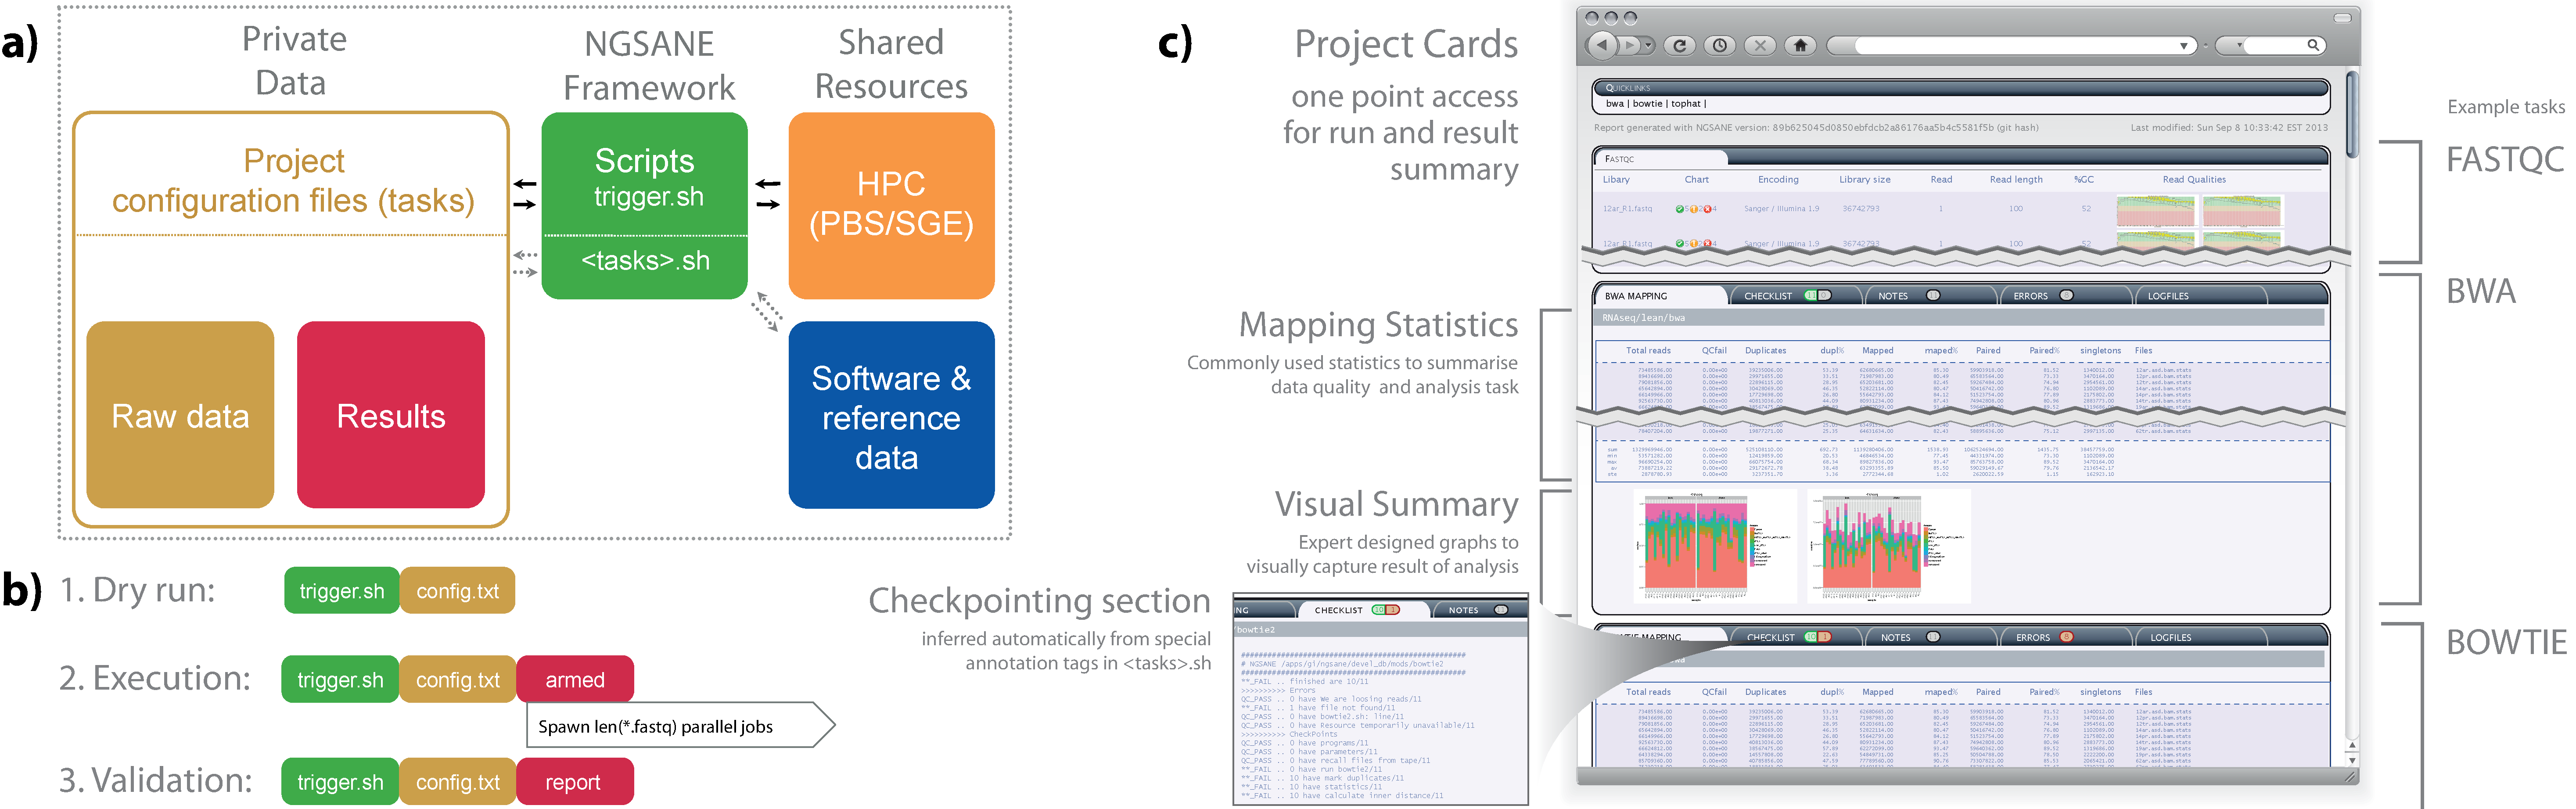
\includegraphics[type=pdf,ext=.pdf,read=.pdf, scale=0.18]{web_screens}
%       \vspace{-0.2cm}
    \caption{
      {\bf a)} Separation of project data from \prog\ core. {\bf b)} Workflow of \prog . {\bf c)} Example of automatically created project summary.} 
      \label{fig:overview}
\end{figure*}

{\it Data security and reusability.}
The framework separates project specific files from reference data, scripts, and software suites that are reusable in other projects (Fig.~\ref{fig:overview}{\bf a}). 
Access to confidential data is handled transparently via the underlying Linux permission system.
The transaction between projects and framework is facilitated by a project specific configuration file that defines paths to reference data as well as the analysis tasks to perform. 
\prog\ supports systems with hierarchical storage management, specifically Data Migration Facility (DMF), by ensuring files are online when needed. 

{\it HPC and parallel execution.} 
\prog\ supports Sun Grid Engine (SGE) and Portable Batch System (PBS) job scheduling and can be operated in different modes for development and production, thus enabling flexible processing of NGS data. 
HPC job partitioning and submission is independent from the program calls, therefore enabling new technologies (e.g. Hadoop) to be incorporated. 

{\it Hot swapping and adaptability.}
Individual task blocks (e.g. read mapping) are packaged in bash script modules, which can be executed locally or on subsets to test module code, submission parameters and compute node environment in stages. 
During production, \prog\ automatically submits separate module calls for each input file or set of files to the HPC queue. 
This allows different existing modules, parameter settings, or software versions to be executed by changes to the project specific configuration file rather than the software code (hot swapping).

{\it Reproducibility and checkpoint recovery.}
A full audit trail is generated recording performed tasks, utilised reference data, timestamps, software version as well as HPC log files, including any errors. 
\prog\ gracefully recovers from unsuccessfully executed jobs be it due to failed commands, missing or incorrect input or under-resourced HPC jobs by cleanly restarting after the most recent successfully executed checkpoint. 

{\it Robust execution and full monitoring.}
In our experience, modular workflows are executed in stages with optional human quality control, \prog\ hence focuses on providing robust checkpointing and intuitive report generation (Fig.~\ref{fig:overview}{\bf b}).
However, workflows can be fully automated by utilising \prog's control over HPC queuing systems and by leveraging the customisable interfaces between modules when submitting multiple dependent stages at once.

{\it Automated project summary creation.}
\prog\ generates a high-level summary (Project Card, Fig.~\ref{fig:overview}{\bf b, c}) to enable informed decisions about the experimental success. 
This interactive HTML report provides an access point for new lab members or collaborators. 
Furthermore, the Project Card can be used as a gold standard for software development when employing a continuous integration server.

{\it Complete customisation.}
\prog's configuration file contains details about the submission system, typical HPC resource allocations and location of third-party software.
However, \prog 's credo is that every parameter can be overwritten, hence default parameters can be adjusted in the project specific configuration file to indicate different software versions, additional resources or an altered output location. 
Additional parameters, such as a specific HPC queue, or new parameters in a software release, can be provided to each program via a special ``free form" variable in the configuration file.  

{\it Repeated calls.}
As stated by \citet{McCoy2013}, pipelines often have to be rerun on the full or a subset of the data with possibly altered parameter settings. 
\prog\ facilitates and documents this by allowing multiple (automatically created) configuration files. 

{\it Knowledge transfer.}
\prog\ provides a unified framework (i.e. folder structure) for processing data from different experimental protocols. 
This allows co-investigators and reviewers to easily understand and reproduce work from \prog 's log and report files. 

\prog\ is open source and available via GitHub.
Currently implemented workflows include those for adapter trimming, read mapping, peak calling, motif discovery, transcript assembly, variant calling and chromatin conformation analysis.
These workflows utilise publicly available published software, yet allow the end user to add their own code and create new workflows as required.
\prog\ is also available as Amazon Machine Image (AMI) and can be deployed to the Amazon Elastic Compute Cloud (EC2) using  {\sc StarCluster} to allow on-demand processing of samples without requiring software installation or HPC maintenance.   

\paragraph{Funding:} 
F.A.B, H.J.F and S.J.C were funded by the National Health and Medical Research Council [1051757, 1010620 and 1063559 to S.J.C]; the Cancer Institute of New South Wales [11/REG/1-10 to Dr Warren Kaplan] and the National Breast Cancer Foundation [program grant to S.J.C.]. Additional funding was received from the Commonwealth Scientific and Industrial Research Organisation's Transformational Capability Platform (D.C.B.), Science and Industry Endowment Fund (D.C.B. and S.J.C) and Information Management and Technology Services.

%APP1063559 Professor Susan Clark SPRF The Garvan Institute of Medical Research $822,925

\paragraph{Acknowledgements:}
Piotr Szul for  help with AMI and StarCluster.

\paragraph{Conflict of Interest:} none declared.
\bibliographystyle{natbib}
\bibliography{ngsane}

\end{document}
